\documentclass[a4paper]{book}
\usepackage{t1enc}
\usepackage[latin1]{inputenc}
\usepackage[french]{minitoc}
 \usepackage{amsmath}
\usepackage{fancyhdr,amsmath,amsthm,amssymb,fancybox}
\usepackage[francais]{babel}
\usepackage{amsmath}
\usepackage{TikZ}
\usetikzlibrary{shapes,backgrounds}
\usepackage{tkz-fct}   
\usepackage{a4wide,jlq2eams} 
\usepackage{graphicx}
\usepackage{hyperref}
\usepackage{slashbox}
\usepackage{thmbox}
\usepackage{xcolor}
\usepackage{sectsty}
\usepackage{longtable} 
\usepackage{multicol}
\usepackage{caption}
\usepackage{pgfplots}
\usepgfplotslibrary{patchplots}
\definecolor{amaranth}{rgb}{0.9, 0.17, 0.31}
\sectionfont{\color{magenta}}
\subsectionfont{\color{red}}
\subsubsectionfont{\color{red}}
\newcommand{\defi}[1]{\textbf{\textcolor{orange}{#1}}}

\setlength{\shadowsize}{1.5pt}
 
\pagestyle{fancy}
\addtolength{\headwidth}{\marginparsep}
\addtolength{\headwidth}{\marginparwidth} 
\renewcommand{\chaptermark}[1]{\markboth{#1}{}}
\renewcommand{\sectionmark}[1]{\markright{\thesection\ #1}}
\fancyhf{}
\fancyhead[LE,RO]{\bfseries\thepage}
\fancyhead[LO]{\bfseries\rightmark}
\fancyhead[RE]{\bfseries\leftmark}
\fancypagestyle{plain}{%
   \fancyhead{} % get rid of headers
   \renewcommand{\headrulewidth}{0pt} % and the line
}

\setcounter{minitocdepth}{3}


\renewcommand{\thesection}{\Roman{section}} 
\renewcommand{\thesubsection}{\Alph{subsection}}
\thmboxoptions{S,bodystyle=\itshape\noindent}
\newtheorem[L]{Lem}{Lemme}[section]
\newtheorem[L]{Th}[Lem]{Th�or�me}
\newtheorem[L]{Cor}[Lem]{Corollaire}
\newtheorem[L]{Prop}[Lem]{Proposition}

\newtheorem[S,bodystyle=\upshape\noindent]{Df}{D�finition}
\newtheorem[S,bodystyle=\upshape\noindent]{Ex}{Exemple}
\newtheorem[S,bodystyle=\upshape\noindent]{NB}{Remarque}
\newtheorem[S,bodystyle=\upshape\noindent]{Methode}{M�thode}
\newtheorem[S,bodystyle=\upshape\noindent]{intr}{Introduction}



\newcommand\SUI{(u_n)_{n\in\N}}
\newcommand\SER{ \sum u_n}
\newcommand\CC[1]{C^{#1}}
\newcommand{\sumni}{\sum_{n=0}^{+\infty}}
\newcommand\Sanxn{ \sum_n a_n x^n}
\newcommand\Sanzn{ \sum_n a_n z^n}
\newcommand\Sbnzn{ \sum_n b_n z^n}
\newcommand\Scnzn{ \sum_n c_n z^n}
\def\abs#1{\mathopen|{#1}\mathclose|}
\def\Abs#1{\left|{#1}\right|}
\newcommand{\Rpinf}{\R \cup \{+\infty\}}
\newcommand\DS{\displaystyle}
\newcommand\To[1]{\xrightarrow[#1]{}}
\newcommand\Toninf{\To{\ninf}}
%%%%%%%%%%%%%%%%%%%%%%%%%%%%





\newcommand{\FIK}{\mathcal{F}(I,\K  )}
\newcommand{\fn}{(f_n)_{n\in \N   }}
\newcommand{\Sfn}{\sum _n f_n}
\newcommand{\TTT}{]a,b]}
\newcommand{\TTTT}{]a,b[}
\newcommand{\me}{e}
\newcommand{\eq}[1]{\mathrm{(#1)}}
\newcommand{\mtag}[1]{\tag{$\mathrm{#1}$}}
\newcommand{\solI}[1]{\mathcal{S}_I(#1)}
\newcommand{\solJ}[1]{\mathcal{S}_J(#1)}
\begin{document}

%https://www.maths-france.fr/MathSpe/Cours/18-fonctions-plusieurs-variables.pdf
%http://math.univ-lyon1.fr/~pujo/analyse3.pdf
%https://perso.univ-rennes1.fr/goulwen.fichou/Cours-VAR-2014.pdf
%C:\Users\tariel\Downloads\cours-mathIV.tex
\chapter{Fonctions de plusieurs variables}
Le cours porte sur les fonctions de plusieurs variables. Prenons un exemple, voici la photographie d'une relief montagneux et sa carte topographique associ�e :\\
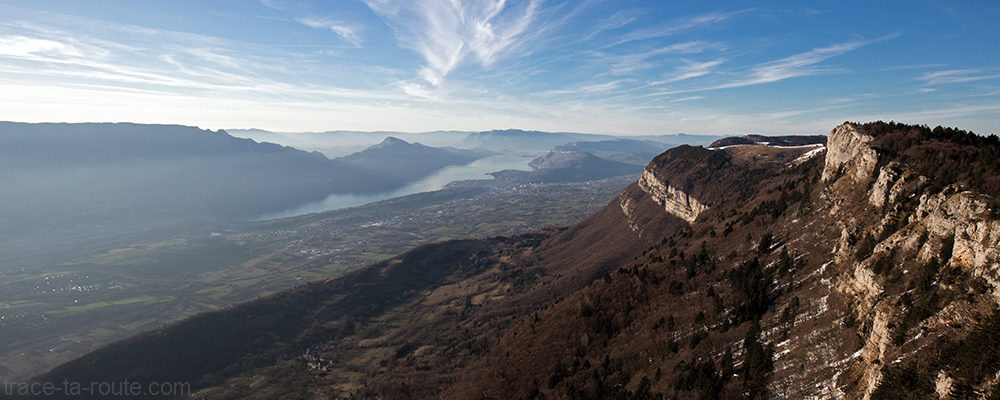
\includegraphics[height=3.5cm]{topography.png}
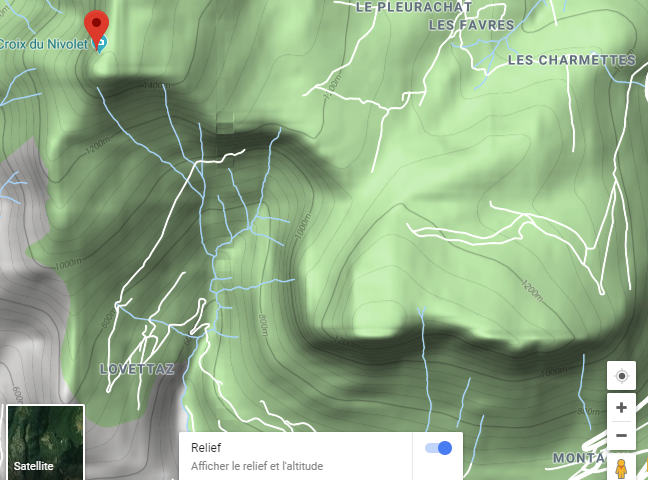
\includegraphics[height=6cm]{topography2.png}.\\
La lecture de la carte de topographique donne l'altitude en fonction de la position d�finie par la latitude et la longitude, soit une fonction d'un domaine $D$ de $\R^2$ � valeurs dans $\R$.  Par exemple, � l'emplacement de la  Croix de Nivolet (45� 3' 49" nord, 5� 57' 56" soit l'ic�ne de localisation en rouge sur la carte), l'altitude donn�e par les courbe de niveaux (points du relief ayant la m�me altitude) est d'� peu pr�s 1500 m�tres. Les falaises repr�sentent des discontinuit� de la fonction. Les cols dans la montagne repr�sentent des points critiques qui ne sont pas des extremum car selon une direction, le col appara�t comme un maximum et selon l'orthogonal de cette direction, comme un minimum.     
\begin{tikzpicture}[scale=0.5]
    \begin{axis}
    \addplot3[patch,patch refines=3,
		shader=faceted interp,
		patch type=biquadratic] 
    table[z expr=x^2-y^2]
    {
        x  y
        -2 -2
        2  -2
        2  2
        -2 2
        0  -2
        2  0
        0  2
        -2 0
        0  0
    };
    \end{axis}
\end{tikzpicture}\\
L'objet de ce cours est d'�tendre l'�tude faite sur les fonctions de la variable r�el aux fonctions de plusieurs variables.

     
D�finitions

Repr�sentation ligne de niveaux graphes voirs cours page 29 http://math.univ-lyon1.fr/~pujo/analyse3.pdf     
     
\begin{tikzpicture}[scale=0.5]
    \begin{axis}
    \addplot3[patch,patch refines=3,
		shader=faceted interp,
		patch type=biquadratic] 
    table[z expr=ln(1+x^2+y^2)]
    {
        x  y
        -10 -10
        10  -10
        10  10
        -2 2
        0  -2
        2  0
        0  2
        -2 0
        0  0
    };
    \end{axis}
\end{tikzpicture}    
Continuit�  


defi
quelques representations voir cours pujo
continuit� technique voir cours maths france



\end{document}

